\documentclass[12pt]{article}
\usepackage{amsmath}
\usepackage{graphicx}
\usepackage{hyperref}
\usepackage{alltt}
\usepackage[utf8]{inputenc}
\usepackage[T1]{fontenc}
\usepackage[brazil]{babel}
\usepackage{graphicx}
\usepackage{fullpage}

\begin{document}

\thispagestyle{empty}

\section*{Diagrama de Classes}

\begin{figure}[htbp]
    \centering 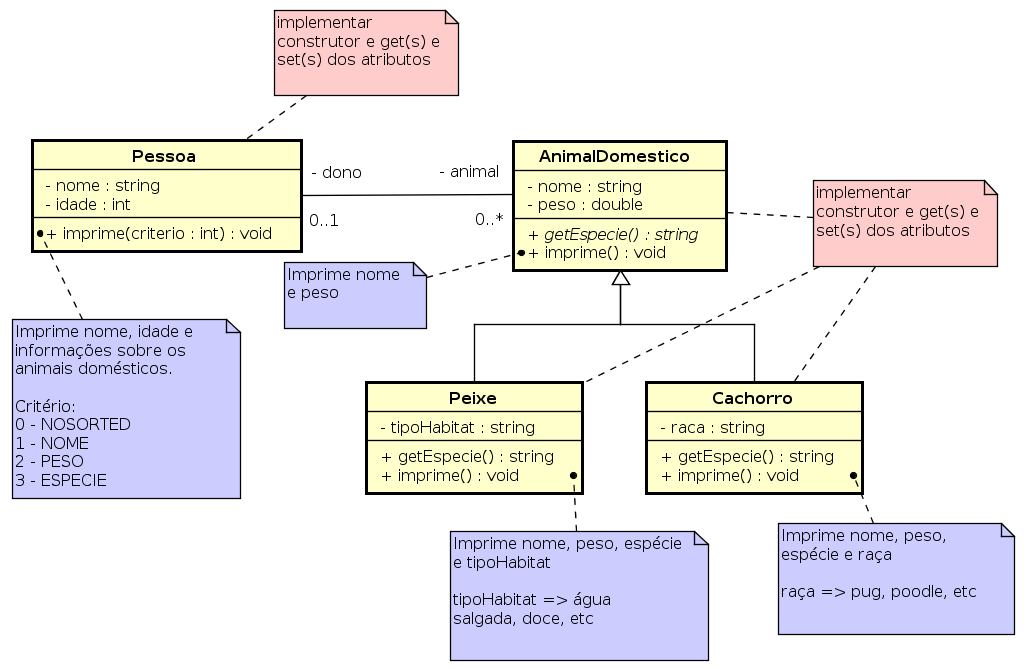
\includegraphics[width=15cm]{animal.png}
\end{figure}

\newpage

\section*{Classe Abstrata {\sf AnimalDomestico}}

\begin{itemize}

\item Atributos: nome ({\sf string}) e peso ({\sf double})

\item Construtor único que inicializa os atributos

\item Métodos {\it getters/setters}

\item Método abstrato {\sf string getEspecie()} a ser implementado pelas subclasses

\item Método {\sf void imprime()} -- que imprime espécie, nome e peso

\end{itemize}

\par\noindent\rule{\textwidth}{0.4pt}

\begin{quote}
\begin{scriptsize}
\begin{verbatim}
#ifndef ANIMALDOMESTICO_H
#define ANIMALDOMESTICO_H

#include <string>
#include <iostream>
using namespace std;

class Pessoa;

class AnimalDomestico {
public:
    AnimalDomestico(string nome, double peso);
    virtual ~AnimalDomestico();
    string getNome() const;
    void setNome(string nome);
    double getPeso() const;
    void setPeso(double peso);
    Pessoa* getDono() const;
    void setDono(Pessoa* dono);
    virtual string getEspecie() = 0;
    virtual void imprime();
    
    static bool compNome(AnimalDomestico* a1, AnimalDomestico* a2);
    static bool compPeso(AnimalDomestico* a1, AnimalDomestico* a2);
    static bool compEspecie(AnimalDomestico* a1, AnimalDomestico* a2);
private:
    Pessoa* dono;
    string nome;
    double peso;
};
#endif /* ANIMALDOMESTICO_H */
\end{verbatim}
\end{scriptsize}
\end{quote}

\par\noindent\rule{\textwidth}{0.4pt}

\begin{quote}
\begin{scriptsize}
\begin{verbatim}
#include "AnimalDomestico.h"

AnimalDomestico::AnimalDomestico(string nome, double peso) :
nome(nome), peso(peso) {
}

AnimalDomestico::~AnimalDomestico() {
}

string AnimalDomestico::getNome() const {
    return nome;
}

void AnimalDomestico::setNome(string nome) {
    this->nome = nome;
}

double AnimalDomestico::getPeso() const {
    return peso;
}

void AnimalDomestico::setPeso(double peso) {
    this->peso = peso;
}

Pessoa* AnimalDomestico::getDono() const {
    return dono;
}

void AnimalDomestico::setDono(Pessoa* dono) {
    this->dono = dono;
}

void AnimalDomestico::imprime() {
    cout << "Espécie: " << this->getEspecie() << endl;
    cout << "Nome: " << this->nome << endl;
    cout << "Peso: " << this->peso << endl;
}

bool AnimalDomestico::compNome(AnimalDomestico* a1, AnimalDomestico* a2) {
    return a1->nome < a2->nome;
}

bool AnimalDomestico::compPeso(AnimalDomestico* a1, AnimalDomestico* a2) {
    return a1->peso < a2->peso;
}

bool AnimalDomestico::compEspecie(AnimalDomestico* a1, AnimalDomestico* a2) {
    if (a1->getEspecie() == a2->getEspecie()) {
        return AnimalDomestico::compNome(a1, a2);
    } else {
        return a1->getEspecie() < a2->getEspecie();
    }
}
\end{verbatim}
\end{scriptsize}
\end{quote}

\par\noindent\rule{\textwidth}{0.4pt}

\newpage

\section*{Classe {\sf Peixe} (subclasse de {\sf AnimalDomestico})}

\begin{itemize}

\item Atributos: tipoHabitat ({\sf string}) -- água doce, água salgada, etc

\item Construtor único que inicializa os atributos       

\item Métodos {\it getters/setters}

\item Método {\sf string getEspecie()} que retorna a string "Peixe"

\item Método {\sf void imprime()} -- que imprime nome, peso, espécie e tipo de habitat

\end{itemize}

\par\noindent\rule{\textwidth}{0.4pt}

\begin{quote}
\begin{scriptsize}
\begin{verbatim}
#ifndef PEIXE_H
#define PEIXE_H

#include "AnimalDomestico.h"

class Peixe : public AnimalDomestico {
public:
    Peixe(string nome, double peso, string habitat);
    virtual ~Peixe();
    string getHabitat() const;
    void setHabitat(string habitat);
    virtual string getEspecie();
    virtual void imprime();
private:
    string habitat;
};

#endif /* PEIXE_H */
\end{verbatim}
\end{scriptsize}
\end{quote}

\par\noindent\rule{\textwidth}{0.4pt}

\begin{quote}
\begin{scriptsize}
\begin{verbatim}
#include "Peixe.h"

Peixe::Peixe(string nome, double peso, string habitat) :
AnimalDomestico(nome, peso), habitat(habitat) {
}

Peixe::~Peixe() {
}

string Peixe::getHabitat() const {
    return habitat;
}

void Peixe::setHabitat(string habitat) {
    this->habitat = habitat;
}

string Peixe::getEspecie() {
    return "Peixe";
}

void Peixe::imprime() {
    AnimalDomestico::imprime();
    cout << "Habitat: " << this->habitat << endl;
}
\end{verbatim}
\end{scriptsize}
\end{quote}

\par\noindent\rule{\textwidth}{0.4pt}

\section*{Classe {\sf Cachorro} (subclasse de {\sf AnimalDomestico})}

\begin{itemize}

\item Atributos: raça ({\sf string}) -- pug, poodle, etc

\item Construtor único que inicializa os atributos

\item Métodos {\it getters/setters}

\item Método {\sf string getEspecie()} que retorna a string "Cachorro"

\item Método {\sf void imprime()} -- que espécie, nome, peso, espécie e raça

\end{itemize}

\par\noindent\rule{\textwidth}{0.4pt}

\begin{quote}
\begin{scriptsize}
\begin{verbatim}
#ifndef CACHORRO_H
#define CACHORRO_H

#include "AnimalDomestico.h"

class Cachorro : public AnimalDomestico {
public:
    Cachorro(string nome, double peso, string raca);
    virtual ~Cachorro();
    string getRaca() const;
    void setRaca(string raca);
    virtual string getEspecie();
    virtual void imprime();
private:
    string raca;
};

#endif /* CACHORRO_H */
\end{verbatim}
\end{scriptsize}
\end{quote}

\par\noindent\rule{\textwidth}{0.4pt}

\begin{quote}
\begin{scriptsize}
\begin{verbatim}
#include "Cachorro.h"

Cachorro::Cachorro(string nome, double peso, string raca) :
AnimalDomestico(nome, peso), raca(raca) {
}

Cachorro::~Cachorro() {
}

string Cachorro::getRaca() const {
    return raca;
}

void Cachorro::setRaca(string raca) {
    this->raca = raca;
}

string Cachorro::getEspecie() {
    return "Cachorro";
}

void Cachorro::imprime() {
    AnimalDomestico::imprime();
    cout << "Raça: " << this->raca << endl;
}
\end{verbatim}
\end{scriptsize}
\end{quote}

\par\noindent\rule{\textwidth}{0.4pt}

\section*{Classe {\sf Pessoa}}

\begin{itemize}

\item Atributos: nome ({\sf string}), idade ({\sf int}) e animais ({\sf vector<AnimalDomestico*>})
       
\item Métodos {\it getters/setters}

\item Métodos para adicionar e remover animais

\begin{itemize}

\item {\sf void adiciona(AnimalDomestico* a)}

\item {\sf void remove(string nome)}

\end{itemize}

\item Método {\sf void imprime()} -- que imprime nome, idade e informações sobre os animais de estimação.

\end{itemize}

\par\noindent\rule{\textwidth}{0.4pt}

\begin{quote}
\begin{scriptsize}
\begin{verbatim}
#ifndef PESSOA_H
#define PESSOA_H

#include "AnimalDomestico.h"
#include <algorithm>
#include <vector>
using namespace std;

enum Criterio { NOSORTED, NOME, PESO, ESPECIE };

class Pessoa {
public:
    Pessoa(string nome, int idade);
    virtual ~Pessoa();
    string getNome() const;
    void setNome(string nome);
    int getIdade() const;
    void setIdade(int idade);
    void adiciona(AnimalDomestico* a);
    void remove(string nome);
    void imprime(Criterio opcao = NOSORTED);
private:
    string nome;
    int idade;
    vector<AnimalDomestico*> animais;
};

#endif /* PESSOA_H */
\end{verbatim}
\end{scriptsize}
\end{quote}

\par\noindent\rule{\textwidth}{0.4pt}

\newpage

\par\noindent\rule{\textwidth}{0.4pt}

\begin{quote}
\begin{scriptsize}
\begin{verbatim}
#include "Pessoa.h"

Pessoa::Pessoa(string nome, int idade) : nome(nome), idade(idade) {}

Pessoa::~Pessoa() {}

string Pessoa::getNome() const { return nome; }

void Pessoa::setNome(string nome) {
    this->nome = nome;
}

int Pessoa::getIdade() const { return idade; }

void Pessoa::setIdade(int idade) {
    this->idade = idade;
}

void Pessoa::adiciona(AnimalDomestico* a) {
    animais.push_back(a);
    a->setDono(this);
}

void Pessoa::remove(string nome) {
    for (int i = 0; i <= animais.size(); i++) {
        AnimalDomestico* animal = animais[i];
        if (animal->getNome() == nome) {
            animais.erase(animais.begin() + i);
            animal->setDono(NULL);
            break;
        }
    }
}

void Pessoa::imprime(Criterio opcao) {
    cout << "========== Pessoa ==========" << endl;
    cout << "Nome:  " << nome << endl;
    cout << "Idade: " << idade << endl;
    if (animais.size() > 0) {
        vector<AnimalDomestico*> copia = animais;
        switch (opcao) {
            case NOME: {
                sort(copia.begin(), copia.end(), AnimalDomestico::compNome);
                break;
            }
            case PESO: {
                sort(copia.begin(), copia.end(), AnimalDomestico::compPeso);
                break;
            }
            case ESPECIE: {
                sort(copia.begin(), copia.end(), AnimalDomestico::compEspecie);
                break;
            }
        }
        for (int i = 0; i < copia.size(); i++) {
            cout << "----------------------------" << endl;
            copia[i]->imprime();
        }
        cout << "----------------------------" << endl;
    }
}
\end{verbatim}
\end{scriptsize}
\end{quote}

\par\noindent\rule{\textwidth}{0.4pt}

\section*{Programa Principal}

Crie o arquivo {\sf main.cpp} com o seguinte conteúdo:

\par\noindent\rule{\textwidth}{0.4pt}

\begin{quote}
\begin{scriptsize}
\begin{verbatim}
#include "Peixe.h"
#include "Pessoa.h"
#include "Cachorro.h"

using namespace std;

int main(int argc, char** argv) {
    
    Pessoa* pessoa = new Pessoa("Joao", 12);
    
    Peixe* nemo = new Peixe("Nemo", 0.15, "Água salgada");
    
    pessoa->adiciona(nemo);
    
    Peixe* dory = new Peixe("Dory", 0.2, "Água doce");
    
    pessoa->adiciona(dory);
    
    Cachorro* teo = new Cachorro("Teo", 6.2, "pug");
    
    pessoa->adiciona(teo);
    
    cout << "================== SEM ORDENAÇÃO ==================" << endl << endl;
    
    pessoa->imprime();
    
    cout << endl;
    
    cout << "================== ORDENAÇÃO (NOME) ==================" << endl << endl;
    
    pessoa->imprime(NOME);
    
    cout << endl;
    
    cout << "================== ORDENAÇÃO (PESO) ==================" << endl << endl;
    
    pessoa->imprime(PESO);
    
    cout << endl;
    
    cout << "================== ORDENAÇÃO (ESPECIE) ==================" << endl << endl;
    
    pessoa->imprime(ESPECIE);
    
    cout << endl;
    
    cout << "================== REMOÇÃO DE UM ELEMENTO ==================" << endl << endl;
        
    pessoa->remove("Dory");
    
    pessoa->imprime();
    
    return 0;
}
\end{verbatim}
\end{scriptsize}
\end{quote}

\par\noindent\rule{\textwidth}{0.4pt}

\end{document}


